\documentclass[aspectratio=169]{beamer}
\usepackage{lmodern}
%\usetheme{Madrid}
%\usecolortheme{giantoak}
\newcommand*\oldmacro{}
\let\oldmacro\insertshorttitle
\renewcommand*\insertshorttitle{\oldmacro\hfill\insertframenumber\,/\,\inserttotalframenumber}
% \newcommand{\light}[1]{\textcolor{gray}{#1}}
%\usepackage{beamerthemesplit}
\usepackage{textpos}
\usepackage{pgf}
\usepackage{ulem}
%\logo{\pgfputat{\pgfxy(0,-.4)}{\pgfbox[right,base]{\includegraphics[height=1.0cm]{logo.jpg}}}}
%\newcommand{\nologo}{\setbeamertemplate{logo}{}}
\usepackage{booktabs}
\usepackage{graphicx}
%\theoremstyle{principle}
%\newtheorem*{principle}{Design Principle}

\title{Limited Dependent Variables}
%\author[Jeremy Kedziora]{\includegraphics[height=2.5cm]{logo.jpg}\\Jeremy Kedziora\\
%\small{Chief Scientist}\\
%\small{Giant Oak}}
\date{\today}

\begin{document}

{
%\nologo
\begin{frame}
    \maketitle
\end{frame}
}


%@@@@@@@@@@@@@@@@@@@@@@@@@@@@@@@@@@@@@@@@@@@@@@@@@@@@@@
\begin{frame}
\frametitle{Objectives}
\begin{itemize}
\item Distinguish between different dependent variable structures;
\bigskip
\bigskip
\item Revisit the assumptions of OLS;
\bigskip
\bigskip
\item Learn (more of) the limitations of OLS;
\end{itemize}
\end{frame}


%@@@@@@@@@@@@@@@@@@@@@@@@@@@@@@@@@@@@@@@@@@@@@@@@@@@@@@
\begin{frame}
\frametitle{So far you've dealt with:}
\begin{enumerate} 

\item Model a linear relationship between dependent variable $y$ and one or more independent variables $x_1,x_2,x_3,\hdots$:
\begin{align*}
y = \beta_0 + \beta_1x_1 + \beta_2x_2 + \beta_3x_3 + \hdots + \varepsilon;
\end{align*}

\item Model a NON-linear relationship between dependent variable $y$ and many independent variables $x$:
\begin{align*}
y = \beta_0 + \beta_1x_1 + \beta_2x_1^2 + \hdots + \varepsilon;
\end{align*}

\item Model relationships between independent variables:
\begin{align*}
y = \beta_0 + \beta_1x_1 + \beta_2x_2 + \beta_{12}x_1x_2 + \varepsilon;
\end{align*}

\item Model pseudo-experimental data using difference in differences.

\end{enumerate}
\end{frame}

%@@@@@@@@@@@@@@@@@@@@@@@@@@@@@@@@@@@@@@@@@@@@@@@@@@@@@@
\begin{frame}
\frametitle{So far you've dealt with:}
\begin{center}
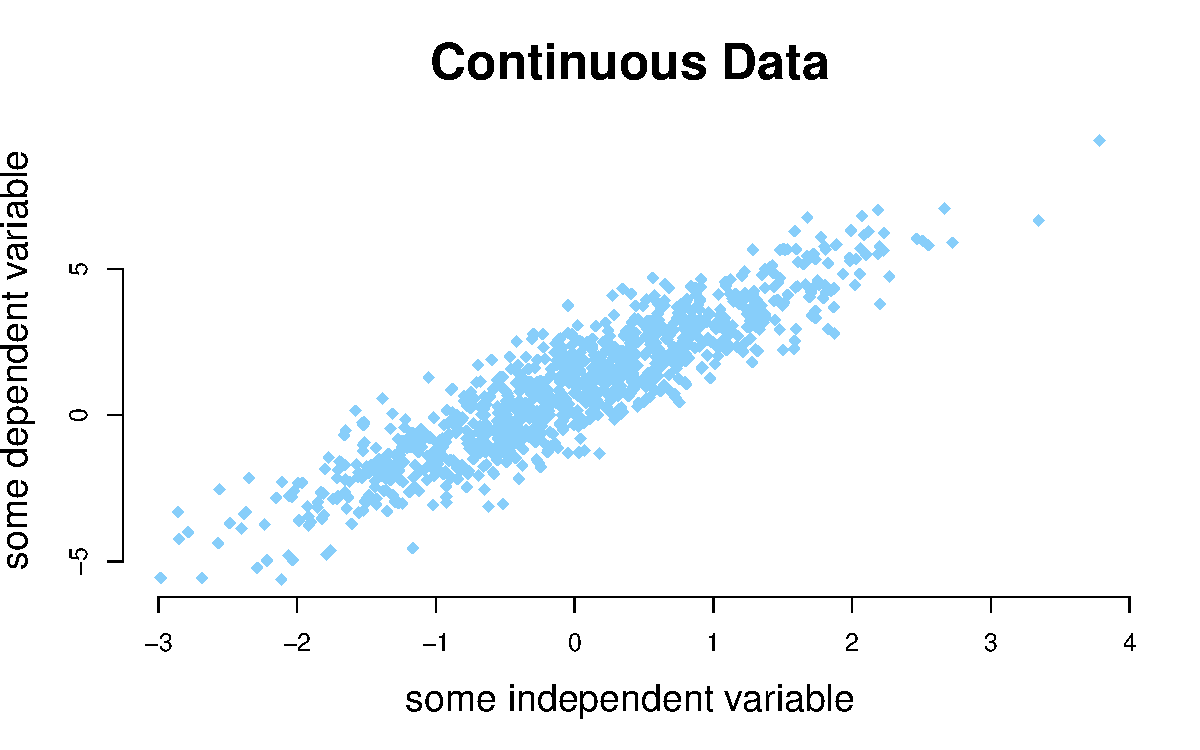
\includegraphics[scale=0.55]{continuous_data.pdf}
\end{center}
\end{frame}

%@@@@@@@@@@@@@@@@@@@@@@@@@@@@@@@@@@@@@@@@@@@@@@@@@@@@@@
\begin{frame}
\frametitle{So far you've dealt with:}
\begin{center}
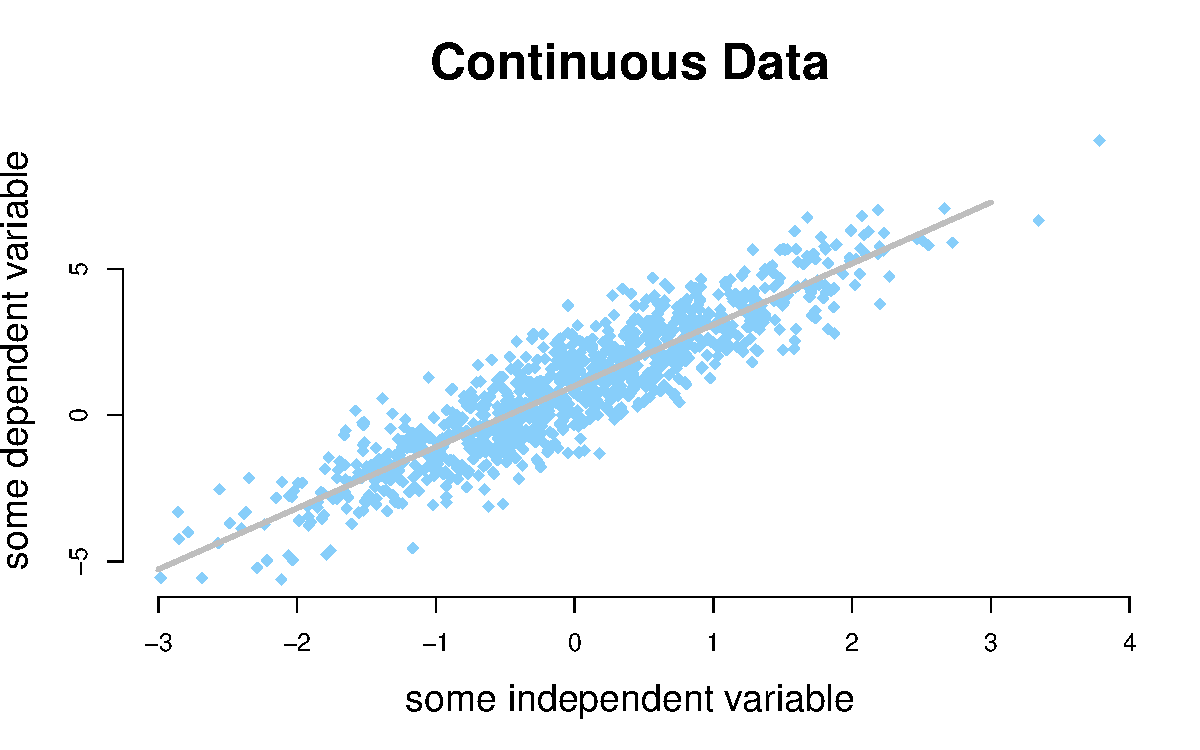
\includegraphics[scale=0.55]{continuous_data_w_line.pdf}
\end{center}
\end{frame}

%@@@@@@@@@@@@@@@@@@@@@@@@@@@@@@@@@@@@@@@@@@@@@@@@@@@@@@
\begin{frame}
\frametitle{So far you've dealt with:}
% latex table generated in R 3.5.1 by xtable 1.8-3 package
% Wed Mar  6 14:49:08 2019
\begin{table}[ht]
\centering
\begin{tabular}{rrrrr}
  \hline
 & Estimate & Std. Error & t value & Pr($>$$|$t$|$) \\ 
  \hline
(Intercept) & 0.9689 & 0.0305 & 31.76 & 0.0000 \\ 
  x & 1.9734 & 0.0301 & 65.57 & 0.0000 \\ 
   \hline
\end{tabular}
\end{table}

\begin{center}\Large
actual relationship: $y = 1 + 2x + \varepsilon$
\end{center}

\end{frame}

%@@@@@@@@@@@@@@@@@@@@@@@@@@@@@@@@@@@@@@@@@@@@@@@@@@@@@@
\begin{frame}
\frametitle{Ok, but what about...}
\begin{center}
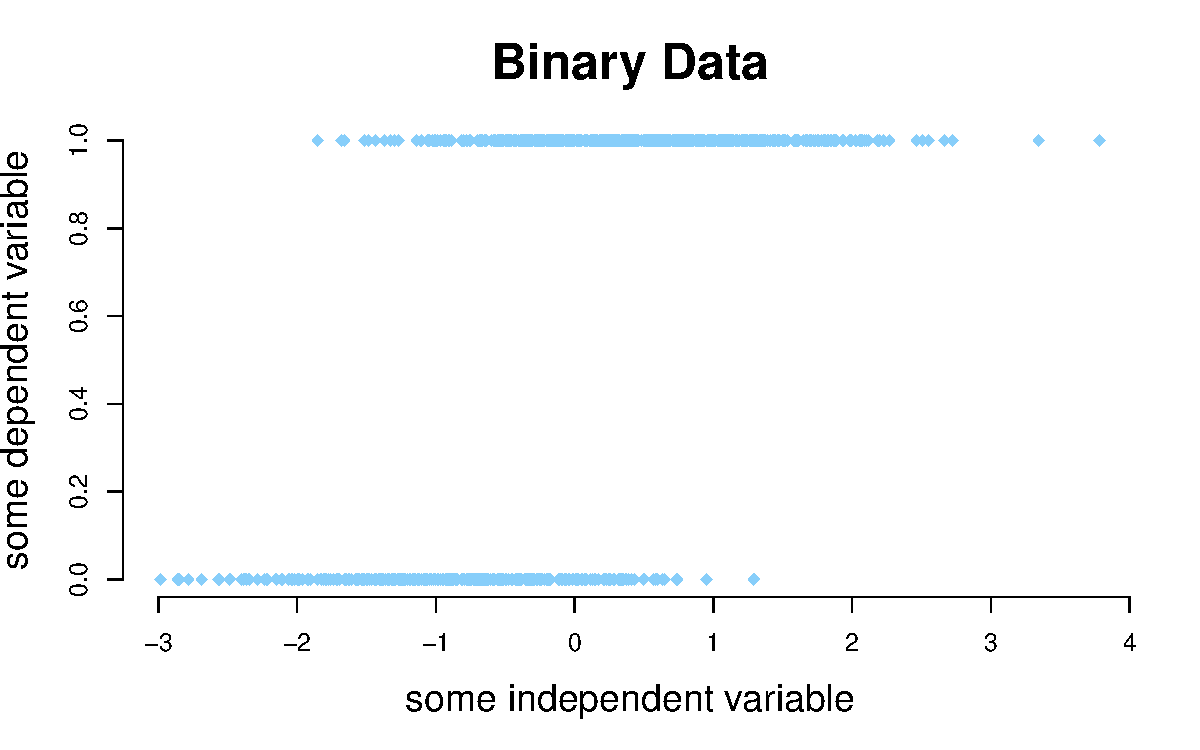
\includegraphics[scale=0.55]{binary_data.pdf}
\end{center}
\end{frame}

%@@@@@@@@@@@@@@@@@@@@@@@@@@@@@@@@@@@@@@@@@@@@@@@@@@@@@@
\begin{frame}
\frametitle{Ok, but what about...}
\begin{center}
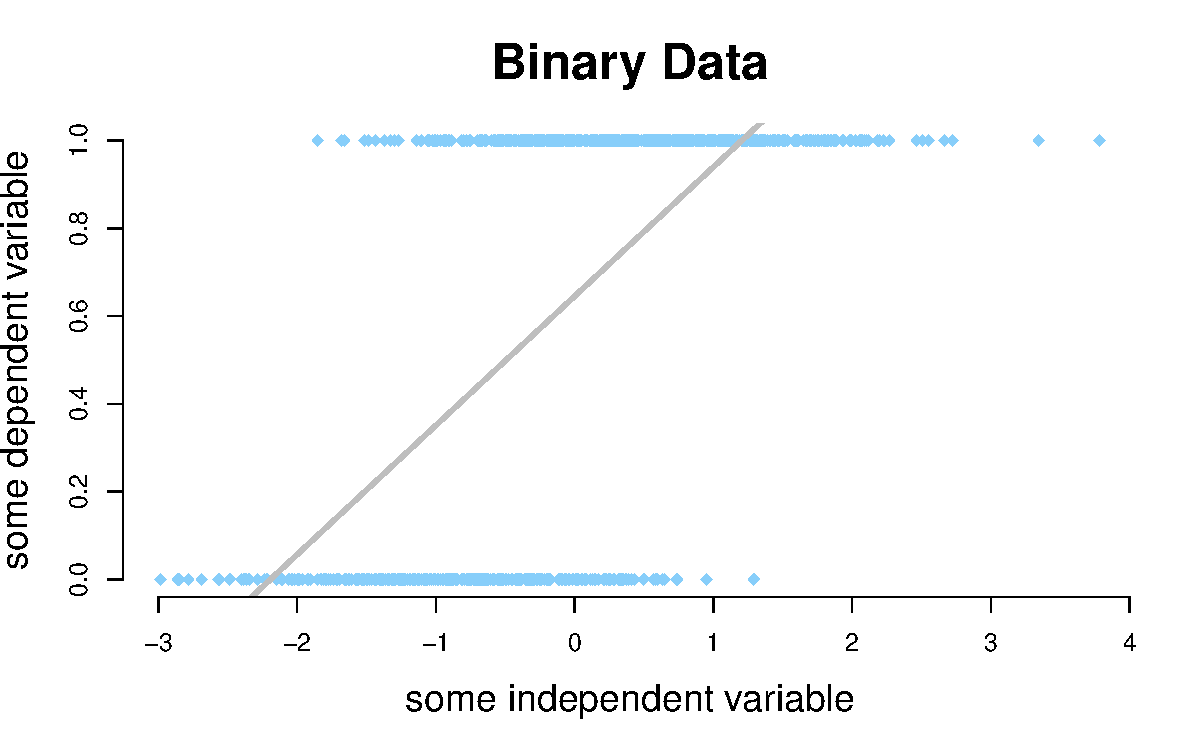
\includegraphics[scale=0.55]{binary_data_w_line.pdf}
\end{center}
\end{frame}

%@@@@@@@@@@@@@@@@@@@@@@@@@@@@@@@@@@@@@@@@@@@@@@@@@@@@@@
\begin{frame}
\frametitle{Ok, but what about...}
% latex table generated in R 3.5.1 by xtable 1.8-3 package
% Wed Mar  6 14:42:46 2019
\begin{table}[ht]
\centering
\begin{tabular}{rrrrr}
  \hline
 & Estimate & Std. Error & t value & Pr($>$$|$t$|$) \\ 
  \hline
(Intercept) & 0.6656 & 0.0123 & 54.21 & 0.0000 \\ 
  x & 0.2630 & 0.0121 & 21.71 & 0.0000 \\ 
   \hline
\end{tabular}
\end{table}

\begin{center}\Large
actual relationship: $y = f(1 + 2x)$... uh oh!
\end{center}

\end{frame}

%@@@@@@@@@@@@@@@@@@@@@@@@@@@@@@@@@@@@@@@@@@@@@@@@@@@@@@
\begin{frame}
\frametitle{And maybe even worse...}

% latex table generated in R 3.5.1 by xtable 1.8-3 package
% Wed Mar  6 15:15:29 2019
\begin{table}[ht]
\centering
\begin{tabular}{rrrrr}
  \hline
 & Estimate & Std. Error & t value & Pr($>$$|$t$|$) \\ 
  \hline
(Intercept) & 18.0014 & 1.8726 & 9.61 & 0.0000 \\ 
  x & 32.1421 & 1.8476 & 17.40 & 0.0000 \\ 
   \hline
\end{tabular}
\end{table}

\begin{center}\Large
actual relationship: $y = f(1 + 2x)$... yikes!
\end{center}

\end{frame}

%@@@@@@@@@@@@@@@@@@@@@@@@@@@@@@@@@@@@@@@@@@@@@@@@@
%{\setbeamercovered{transparent}
\begin{frame}
\frametitle{So can't we just use OLS?}
Why do we choose to use OLS?  Because... \onslide<2-> when its assumptions are satisfied it's BLUE!

\begin{enumerate}
\item Dependent variable is a \textbf{linear} function of independent variables plus noise;
\begin{align*}
y = \beta_0 + \beta_1x_1 + \beta_2x_2 + \hdots + \beta_mx_m + \varepsilon
\end{align*}

\item Independent variables are not related to each other -- \textbf{no multicollinearity};
\bigskip

\item Independent variables have \textbf{no measurement error};
\bigskip

\item Noise term is a random variable following the \textbf{normal distribution};
\bigskip

\item[]
\end{enumerate}

\end{frame}
%}

%@@@@@@@@@@@@@@@@@@@@@@@@@@@@@@@@@@@@@@@@@@@@@@@@@@@@@@
\begin{frame}
\frametitle{So can't we just use OLS?}
Why do we choose to use OLS?  Because...  when its assumptions are satisfied it's BLUE!
\begin{center}
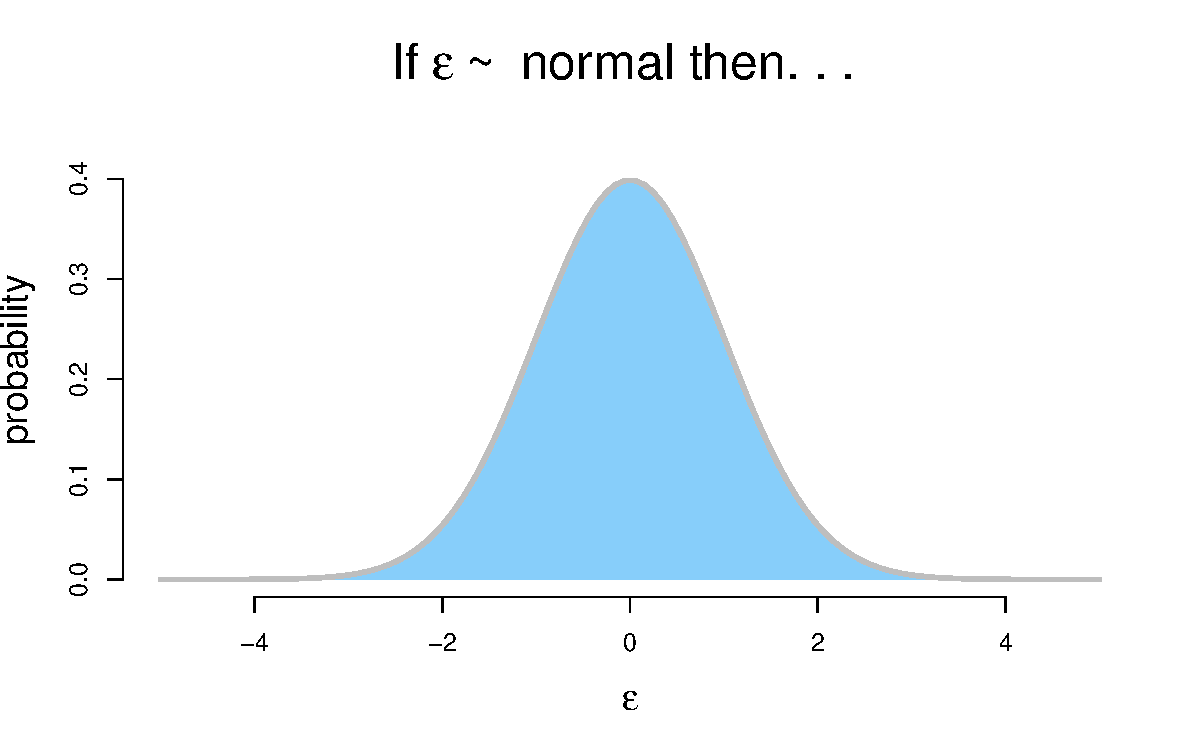
\includegraphics[scale=0.55]{normal_distribution.pdf}
\end{center}
\end{frame}

%@@@@@@@@@@@@@@@@@@@@@@@@@@@@@@@@@@@@@@@@@@@@@@@@@@@@@@
\begin{frame}
\frametitle{So can't we just use OLS?}
Why do we choose to use OLS?  Because...  when its assumptions are satisfied it's BLUE!
\begin{center}
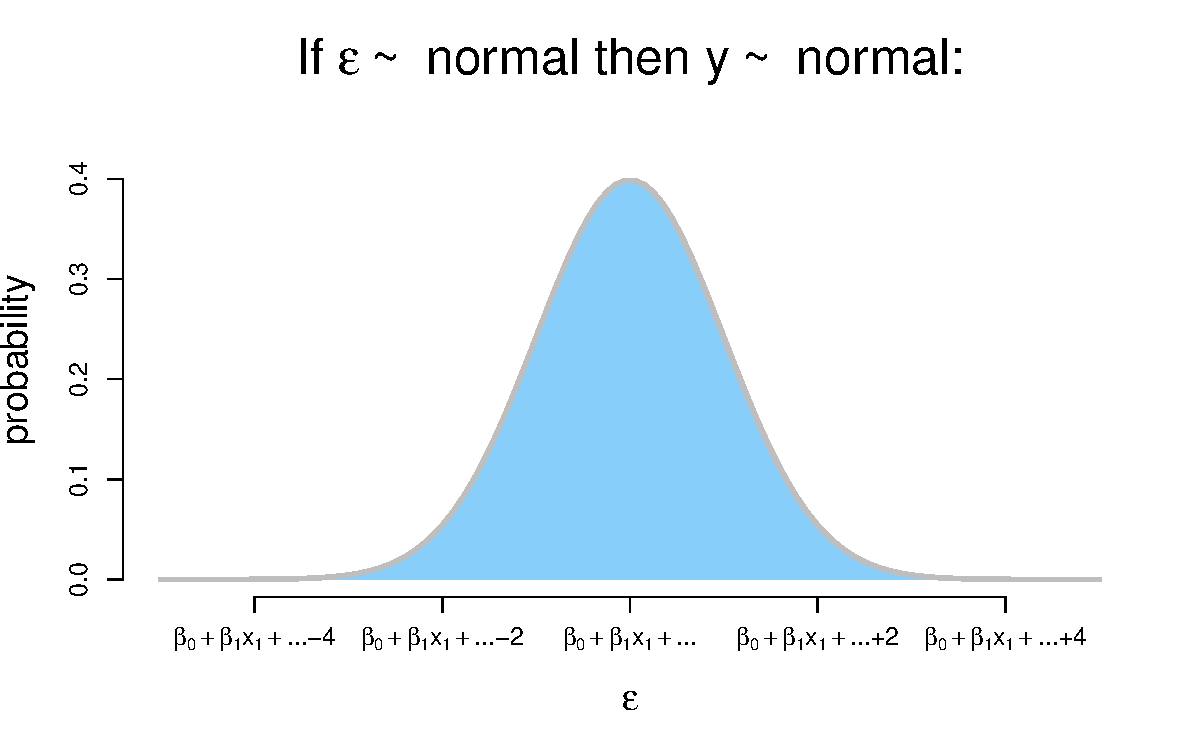
\includegraphics[scale=0.55]{normal_distribution_y.pdf}
\end{center}
\end{frame}

%@@@@@@@@@@@@@@@@@@@@@@@@@@@@@@@@@@@@@@@@@@@@@@@@@@@@@@
\begin{frame}
\frametitle{What does this mean? On the theory side:}
\begin{itemize}
\item The \textbf{linear function} and \textbf{normal errors} assumptions require that $y$ be able to take on any value!
\bigskip
\bigskip
\item If the dependent variable is binary, i.e. always either 0 or 1 then...
\bigskip
\begin{enumerate}
\item either \textbf{linear function} or \textbf{normal errors} are \textbf{wrong}, or...
\bigskip
\item something exceedingly unlikely happened.
\bigskip
\end{enumerate}
\end{itemize}
\end{frame}

%@@@@@@@@@@@@@@@@@@@@@@@@@@@@@@@@@@@@@@@@@@@@@@@@@@@@@@
\begin{frame}
\frametitle{What does this mean? On the practical side:}
\begin{center}
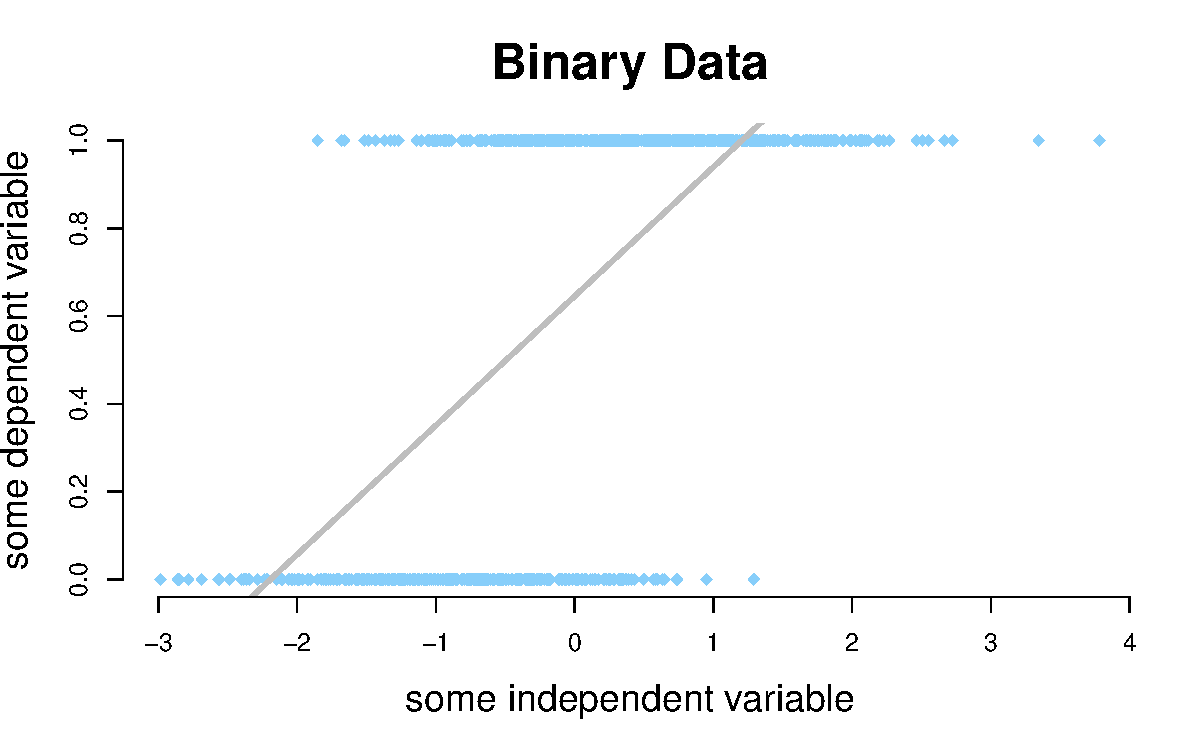
\includegraphics[scale=0.55]{binary_data_w_line.pdf}
\end{center}
\end{frame}

%@@@@@@@@@@@@@@@@@@@@@@@@@@@@@@@@@@@@@@@@@@@@@@@@@@@@@@
\begin{frame}
\frametitle{What does this mean? On the practical side:}
% latex table generated in R 3.5.1 by xtable 1.8-3 package
% Wed Mar  6 14:42:46 2019
\onslide<1->\begin{table}[ht]
\centering
\begin{tabular}{rrrrr}
  \hline
 & Estimate & Std. Error & t value & Pr($>$$|$t$|$) \\ 
  \hline
(Intercept) & 0.6656 & 0.0123 & 54.21 & 0.0000 \\ 
  x & 0.2630 & 0.0121 & 21.71 & 0.0000 \\ 
   \hline
\end{tabular}
\end{table}
\bigskip

\onslide<1-> \begin{center}Let's use this to make predictions...  \end{center}
\setbeamercovered{invisible}
\begin{table}
\begin{tabular}{r | c | c }
If $x=$ & $y = 0.6656 + 0.2630x$ & then $y =$ ... \onslide<1-> \\
\hline \hline
$0$ & $y = 0.6656 + 0.2630*0$ & $0.6656$  \onslide<2-> \\ 
$1$ & $y = 0.6656 + 0.2630*1$ & $0.9286$  \onslide<2-> \\ 
$2$ & $y = 0.6656 + 0.2630*2$ & $1.1916$  \onslide<2-> \\ 
$-3$ & $y = 0.6656 + 0.2630*(-3)$ & $-0.1234$  \onslide<2-> \\ 
%Norman P & 8:00 & 22:45 & 23:02 & 53:47 \onslide<4->\\
%Alex K & 14:00 & 28:00 & n/a & n/a \onslide<5->\\
%Sarah H & 9:22 & 21:10 & 24:03 & 54:35 
\end{tabular}
\end{table}
\onslide<3->\begin{center}Leads to nonsense!\end{center}
\end{frame}

%@@@@@@@@@@@@@@@@@@@@@@@@@@@@@@@@@@@@@@@@@@@@@@@@@@@@@@
\begin{frame}
\frametitle{What does this mean?  OLS is not the best model.}
\begin{center}
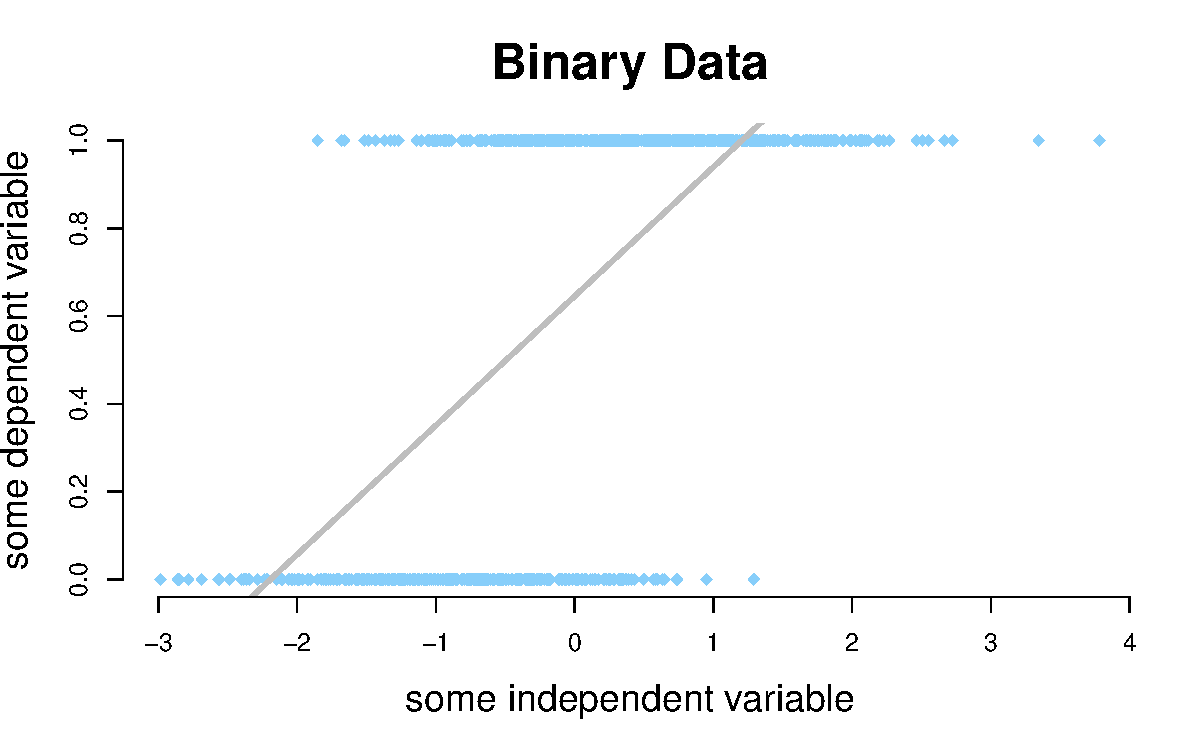
\includegraphics[scale=0.55]{binary_data_w_line.pdf}
\end{center}
\end{frame}

%@@@@@@@@@@@@@@@@@@@@@@@@@@@@@@@@@@@@@@@@@@@@@@@@@@@@@@
\begin{frame}
\frametitle{What does this mean?  OLS is not the best model.}
\begin{center}
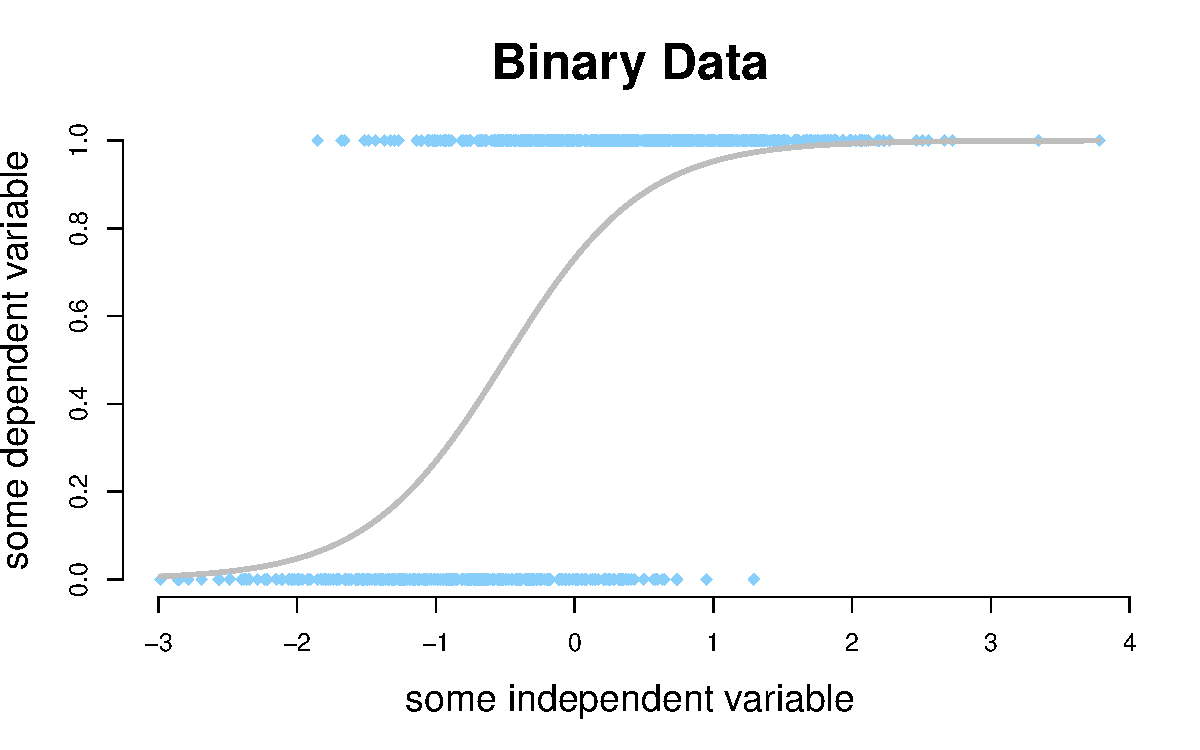
\includegraphics[scale=0.55]{binary_data_w_s_curve.pdf}
\end{center}
\end{frame}

%@@@@@@@@@@@@@@@@@@@@@@@@@@@@@@@@@@@@@@@@@@@@@@@@@@@@@@
\begin{frame}
\frametitle{So how do we deal with this?}
A very general way of addressing this type of problem (weird dependent variable) is to use a \textbf{Generalized Linear Model} (GLM).\\
\bigskip
\bigskip
\onslide<2-> GLMs have three required components:
\begin{enumerate}
\item A probability distribution that describes the dependent variable;
\item A linear model $\beta_0 + \beta_1x_1 + \beta_2x_2 + ...$;
\item A link function that relates the linear model to the dependent variable distribution.
\end{enumerate}
\bigskip

Binary data: GLM = Logistic regression;
\end{frame}

%@@@@@@@@@@@@@@@@@@@@@@@@@@@@@@@@@@@@@@@@@@@@@@@@@
\begin{frame}

\begin{center}
\Huge\textbf{Why should we care?}\\
\bigskip
\bigskip
\large Limited dependent variables require different modeling strategies -- we'll explore one of them next week.\\
\end{center}

\end{frame}


\end{document}

